\vspace{-3mm}
\section{ALOHA}
\vspace{-1mm}
\subsection{PURE ALOHA}
가장 기본적인 random access protocols이다. Shared Network 에서 어떤 device가 전송을 random 시간에 의존해서 ACK 신호를 보내고, 이를 수신받지 못하는 상황을 collison이 발생한다고 인지한다. 그럼 해당 네트워크에 접속한 이후  collison 횟수를 count 하고, count 수를 $k$라고 할때 0 부터 $2^{k-1}$의 대기시간을 가지며 재전송을 진행한다.  이렇게 BEB\footnote{binary exponential backoff}로 재전송시간 term을 정해주면 언젠가는 collison이 일어나지 않을것이다. \\
\vspace{-4mm}  
    \begin{figure}[!h]\centering
		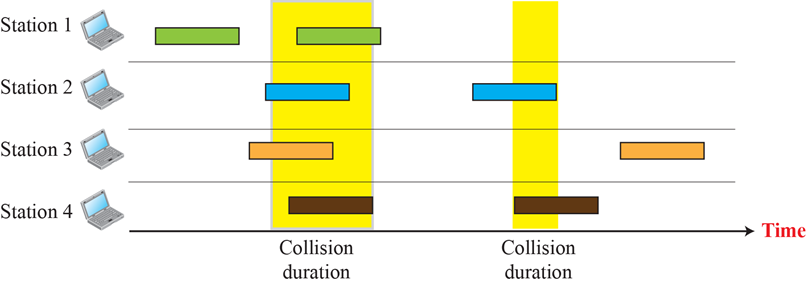
\includegraphics[width=.66\textwidth]{image/week12/1-1.png}
% 		\caption*{\small }
		\vspace{-10pt}
    \end{figure}
\vspace{-4mm}

\subsection{SLOTTED ALOHA}
Slotted Aloha는 Pure Aloha의 높은 Collison 발생가능성을 개선하기 위해 고안된 protocols이다. Slot이란말 그대로 Pure Aloha에서 전송가능한 시간의 space가 연속적이었다면 , 이를 일정한 timestep을 가지는 step으로 제한하여 각 slot 시간 사이에서 전송을 하고자 하는 device의 frame 전송시간을 각각 slot 사이로 특정함으로서 collison 확률의 발생을 줄인 protocols이다.
\vspace{-4mm}  
    \begin{figure}[!h]\centering
		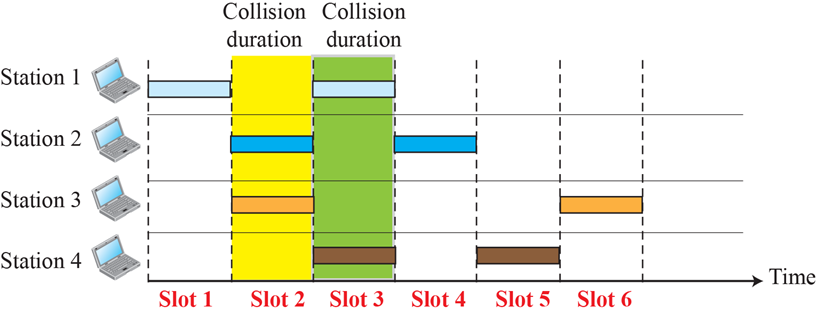
\includegraphics[width=.66\textwidth]{image/week12/1-2.png}
% 		\caption*{\small }
		\vspace{-10pt}
    \end{figure}
\clearpage
\subsection{Comparison of throughput between pure-aloha and slotted-aloha}
% \vspace{-2mm}
Throughpput은 단위시간동안 보내는 packet의 개수로, 성공적인 Frame 전송의 평균값을 의미한다.
\vspace{-4mm}
\subsubsection*{Vulnerable Time : Pure Aloha}
\vspace{-2mm}
shared link에서 한 device가 전송중에 있으면 다른 device또한 이시간동안은 다른 device에서도 전송을 하면 collision이 발생하게 된다. Vulnerable time은 한 device가 어느 구간에서 어느 구간까지 전송이 없어야 성공적으로 frame을 보낼 수 있는지 판단하는 최소의 단위다.
이때 문제를 단순화하고 2 aloha protocol을 비교하기 위해서 단위를 통일시켜보자. 각 frame이 전송되는 시간을 $T_{fr}$  이고 모든 device에서 동일하다고 할때, Pure Aloha에서는  figure와 같이 전송시간이 정해지지 않았기때문에 collison 이 발생할 수 있는 time domain은 2개의 frame의 전송시간의 합인 $2T_{fr}$이 vulnerable time이 된다.
\vspace{-4mm}  
    \begin{figure}[!h]\centering
		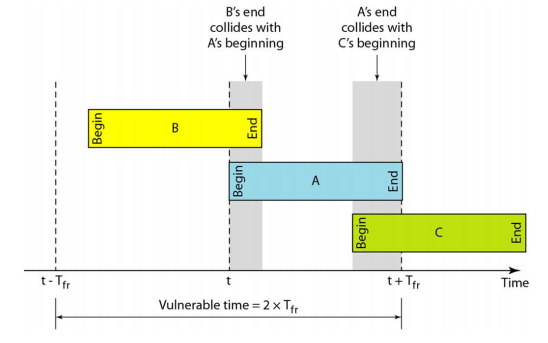
\includegraphics[width=.55\textwidth]{image/week12/1-3.png}
% 		\caption*{\small }
		\vspace{-10pt}
    \end{figure}
\vspace{-4mm}
\subsubsection*{Vulnerable Time : Slotted Aloha}
\vspace{-2mm}
반면 slotted aloha에서는 각 frame의 전송시간이 $T_{fr}$로 통일될때, 최적의 slot 길이는 $T_{fr}$ 이므로 slotted aloha 의 vulnerable time은 $T_{fr}$ 이다. 
\vspace{-2mm}
\subsubsection*{Throughput}
\vspace{-2mm}
Throughput은 아래의 equation과 같이 표현할 수 있다. 이때 $G-\text{load}$ 는 주어진시간동안 전송을 시도한 평균횟수이다. 
$$
S(\text{throughput}) = P_{success} \times G-\text{load}
$$
일정시간동안 발생하는 횟수에 관한 문제이므로, frame을 한 device에서 전송하는 과정을 poison process로 모델링 할 수 있다.이때 전송을 시도하는 확률을 $\lambda$ 라고할때,   T 시간동안 K번 frame이 도착하는 $P_{success}$ 는 $P[\text{k arrivals in T seconds}] = \frac{(\lambda T)^k}{k!} e^{-\lambda T}$로 표현할 수 있다.  $\lambda$ 는 앞서 정의해준 G-load에서 성공할 수 있는 최소의 단위시간인 vulnerable time 으로 나눈값으로  표현할 수 있으므로, 
